%%%%%%%%%%%%%%%%%%%%%%%%%%%%%%%%%%%%%%%%%
% University/School Laboratory Report
% LaTeX Template
% Version 4.0 (March 21, 2022)
%
% This template originates from:
% https://www.LaTeXTemplates.com
%
% Authors:
% Vel (vel@latextemplates.com)
% Linux and Unix Users Group at Virginia Tech Wiki
%
% License:
% CC BY-NC-SA 4.0 (https://creativecommons.org/licenses/by-nc-sa/4.0/)
%
%%%%%%%%%%%%%%%%%%%%%%%%%%%%%%%%%%%%%%%%%

%----------------------------------------------------------------------------------------
%	PACKAGES AND DOCUMENT CONFIGURATIONS
%----------------------------------------------------------------------------------------

\documentclass[
	letterpaper, % Paper size, specify a4paper (A4) or letterpaper (US letter)
	10pt, % Default font size, specify 10pt, 11pt or 12pt
]{CSUniSchoolLabReport}

%----------------------------------------------------------------------------------------
%	REPORT INFORMATION
%----------------------------------------------------------------------------------------

\title{ECE 398-MA \\ Introduction to Modern Communication with Python and SDR \\ Lab 8 -- FSK} % Report title

\author{Noah Breit} % Author name(s), add additional authors like: '\& James \textsc{Smith}'

\date{\today} % Date of the report

%----------------------------------------------------------------------------------------

\begin{document}

\maketitle % Insert the title, author and date using the information specified above

% \begin{center}
% 	\begin{tabular}{l r}
% 		Date Performed: & February 13, 2022 \\ % Date the experiment was performed
% 		Partners: & Cecilia \textsc{Smith} \\ % Partner names
% 		& Tajel \textsc{Khumalo} \\
% 		Instructor: & Professor \textsc{Rivera} % Instructor/supervisor
% 	\end{tabular}
% \end{center}

% If you need to include an abstract, uncomment the lines below
%\begin{abstract}
%	Abstract text
%\end{abstract}

%----------------------------------------------------------------------------------------
%	OBJECTIVE
%----------------------------------------------------------------------------------------

\section{Assignment 1}

\begin{lstlisting}[language=Python]
	import numpy as np
	import matplotlib.pyplot as plt
	
	## Parameters
	fs = 1000  # Sampling rate (Hz)
	fc = 100   # Carrier frequency (Hz)
	Tb = 1     # Symbol duration (s)
	N = int(fs * Tb)  # Samples per symbol
	t = np.linspace(0, Tb, N, endpoint=False)
	
	## FSK Signal Generation
	def generate_2fsk_signal(syms, fc, delta_f):
	signal = []
	for sym in syms:
	f = fc + (2 * sym - 1) * delta_f / 2  # Choose f0 or f1
	s = np.sqrt(2/Tb)*np.cos(2*np.pi*f*t)
	signal.extend(s)
	return np.array(signal)
	
	######################## PART ONE ##############################
	delta_f = 1/Tb
	phi0 = generate_2fsk_signal([0], fc, delta_f)
	phi1 = generate_2fsk_signal([1], fc, delta_f)
	
	# matplotlib time domain plot
	plt.figure(figsize=(12, 6))
	plt.subplot(1, 2, 1)
	plt.plot(t[:100], phi0[:100], label='Phi_0 (0)')
	plt.plot(t[:100], phi1[:100], label='Phi_1 (1)')
	plt.title('First 100 Samples')
	plt.xlabel('Time (s)')
	plt.ylabel('Amplitude')
	plt.legend()
	plt.savefig('phi_time_domain.png')
	plt.grid()
	
	# matplotlib freq domain plot
	plt.subplot(1, 2, 2)
	for sig, label in [(phi0, 'Phi_0'), (phi1, 'Phi_1')]:
	fft_result = np.fft.fftshift(np.fft.fft(sig))
	freq = np.fft.fftshift(np.fft.fftfreq(len(sig), 1/fs))
	plt.plot(freq, np.abs(fft_result)/len(sig), label=label)
	
	plt.xlim(50, 150)
	plt.title('Spectrum')
	plt.xlabel('Frequency (Hz)')
	plt.ylabel('Magnitude')
	plt.legend()
	plt.grid()
	plt.tight_layout()
	plt.savefig('phi_freq_domain.png')
	plt.show()
\end{lstlisting}

\begin{figure}[H] % [H] forces the figure to be placed exactly where it appears in the text
	\centering % Horizontally center the figure
	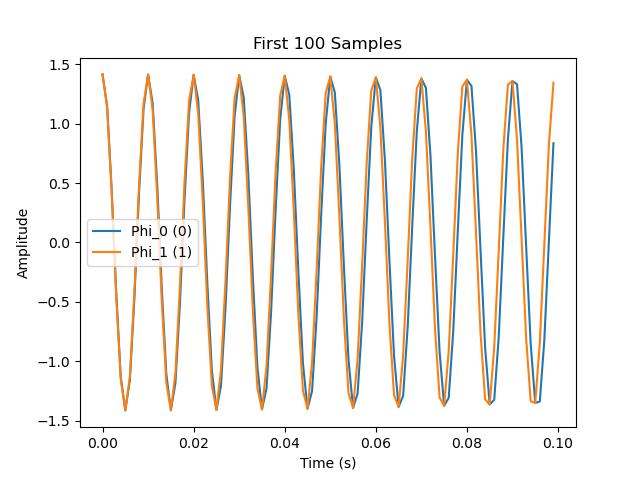
\includegraphics[width=1.2\textwidth]{phi_time_domain.png} % Include the figure
	\caption{FSK Symbols Time Domain}
	\label{fig:block}
\end{figure}

\begin{figure}[H] % [H] forces the figure to be placed exactly where it appears in the text
	\centering % Horizontally center the figure
	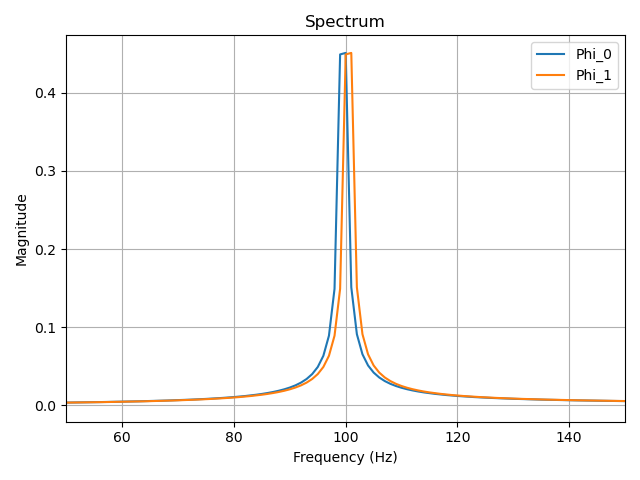
\includegraphics[width=1.2\textwidth]{phi_freq_domain.png} % Include the figure
	\caption{FSK Symbols Frequency Domain}
	\label{fig:block}
\end{figure}

\begin{lstlisting}[language=Python]
	######################## PART TWO ############################
	num_syms = 128
	syms = np.random.randint(0, 2, num_syms)
	
	# Generate FSK signal
	delta_f = (1.0 / Tb)
	signal = generate_2fsk_signal(syms, fc, delta_f)
	
	# Add AWGN
	noise_amplutide = 0.1
	noise = noise_amplutide * np.random.randn(len(signal))
	rx_signal = signal + noise
	
	## Detection Implementations
	def coherent_detection_2fsk(rx_signal, fc, delta_f, theta):
	ys = np.empty((0,2))    # observation vectors
	syms = np.array([])     # recoered symbols (0 or 1)
	
	# create two orthonormal basis
	
	# the original transmitted symbol points (each is a 2-dim vector)
	s0 = np.array([1, 0])
	s1 = np.array([0, 1])
	
	# create two orthonormal basis with the phase offsets 
	# (theta[0] for phi0, theta[1] for pho1)
	# phi0_theta = phi0 * np.exp(2*np.pi*theta[0])
	# phi1_theta = phi1 * np.exp(2*np.pi*theta[1])
	phi0_theta = np.sqrt(2/Tb)*np.cos(2*np.pi*(fc - delta_f/2)*t + theta[0])
	phi1_theta = np.sqrt(2/Tb)*np.cos(2*np.pi*(fc + delta_f/2)*t + theta[1])
	
	for i in range(0, len(rx_signal), N):
	# received signal in Tb duration
	segment = rx_signal[i:i+N]
	# if len(segment) < N: continue
	
	# compute the y vector coefficients
	y0 = np.dot(segment, phi0_theta)/fs
	y1 = np.dot(segment, phi1_theta)/fs
	
	y = np.array([y0, y1])
	ys = np.vstack([ys, y])
	
	# make decisions by choosing the closest distance (use linalg.norm)
	decision = np.argmin([np.linalg.norm(y - s0), np.linalg.norm(y - s1)])
	syms = np.append(syms, decision)
	
	return ys, syms
	
	def noncoherent_detection_2fsk(rx_signal, fc, delta_f, theta):
	ys = np.empty((0,2))    # observation vectors
	syms = np.array([])     # recoered symbols (0 or 1)
	
	# create two orthonormal basis
	
	# the original transmitted symbol points (each is a 2-dim vector)
	s0 = np.array([1, 0])
	s1 = np.array([0, 1])
	
	# create two orthonormal basis (and its quadrature) with the phase offsets
	# (theta[0] for phi0, theta[1] for phi1)
	phi0_theta = np.sqrt(2/Tb)*np.cos(2*np.pi*(fc - delta_f/2)*t + theta[0])
	phi0Q_theta = -1*np.sqrt(2/Tb)*np.sin(2*np.pi*(fc - delta_f/2)*t + theta[0])
	phi1_theta = np.sqrt(2/Tb)*np.cos(2*np.pi*(fc + delta_f/2)*t + theta[1])
	phi1Q_theta = -1*np.sqrt(2/Tb)*np.sin(2*np.pi*(fc + delta_f/2)*t + theta[1])
	
	for i in range(0, len(rx_signal), N):
	# received signal in Tb duration
	segment = rx_signal[i:i+N]
	
	# Compute the y vector coefficients
	y0_I = np.dot(segment, phi0_theta)/fs
	y0_Q = np.dot(segment, phi0Q_theta)/fs
	y1_I = np.dot(segment, phi1_theta)/fs
	y1_Q = np.dot(segment, phi1Q_theta)/fs
	
	y0 = np.sqrt(y0_I**2 + y0_Q**2)
	y1 = np.sqrt(y1_I**2 + y1_Q**2)
	
	y = np.array([y0, y1])
	ys = np.vstack([ys, y])
	
	# make decision by choosing the closest distance (use linalg.norm)
	decision = np.argmin([np.linalg.norm(y - s0), np.linalg.norm(y - s1)])
	syms = np.append(syms, decision) 
	
	return ys, syms
	
	# Phase offset experiment
	thetas = [
	[0, 0],
	[np.pi/2, np.pi/2],
	np.random.uniform(-np.pi, np.pi, 2),
	np.random.uniform(-np.pi, np.pi, 2),
	np.random.uniform(-np.pi, np.pi, 2)
	]
	
	for idx, theta in enumerate(thetas):
	print(f"\nTheta: {theta}")
	y_coh, sym_coh = coherent_detection_2fsk(rx_signal, fc, delta_f, theta)
	y_noncoh, sym_noncoh = noncoherent_detection_2fsk(rx_signal, fc, delta_f, theta)
	
	# DEBUG
	# print(y_coh[:10])
	
	ser_coh = 100*np.mean(syms != sym_coh)
	ser_noncoh = 100*np.mean(syms != sym_noncoh)
	
	print('Symbol error rate (coherent demod) (%): ', 100*np.count_nonzero(syms != sym_coh)/num_syms)
	print('Symbol error rate (non-coherent demod) (%): ', 100*np.count_nonzero(syms != sym_noncoh)/num_syms)
	
	# Constellation plot
	plt.figure()
	plt.plot(y_coh[:,0], y_coh[:,1], 'o', label='coherent')
	plt.plot(y_noncoh[:,0], y_noncoh[:,1], 'o', label='non-coherent')
	plt.axhline(0, color='black')
	plt.axvline(0, color='black')
	plt.grid()
	plt.xlim([-2, 2])
	plt.ylim([-2, 2])
	plt.legend()
	ax = plt.gca()
	ax.set_aspect('equal', adjustable='box')
	plt.xlabel(r'$\mathrm{\phi_0(t)}$')
	plt.ylabel(r'$\mathrm{\phi_1(t)}$')
	plt.title('Constellation')
	plt.savefig(f'phase_offset{idx}.png')
	plt.show()
	
	# Frequency separation impact
	delta_fs = [1.0/Tb, 1.0/(2*Tb), 10.5/Tb]
	for idx, df in enumerate(delta_fs):
	signal = generate_2fsk_signal(syms, fc, df)
	noise = noise_amplutide * np.random.randn(len(signal))
	rx_signal = signal + noise
	
	_, sym_noncoh = noncoherent_detection_2fsk(rx_signal, fc, df, [0,0])
	y_noncoh, _ = noncoherent_detection_2fsk(rx_signal, fc, df, [0,0])
	
	plt.figure()
	plt.plot(y_noncoh[:,0], y_noncoh[:,1], 'o')
	plt.title(f'Non-coherent Constellation (delta_f={df:.2f} Hz)')
	plt.xlabel('Phi_0(t)')
	plt.ylabel('Phi_1(t)')
	plt.grid()
	plt.axis('equal')
	plt.savefig(f'freq_separation{idx}.png')
	plt.show()
\end{lstlisting}

Phase Offset Experiment:\newline

\begin{figure}[H] % [H] forces the figure to be placed exactly where it appears in the text
	\centering % Horizontally center the figure
	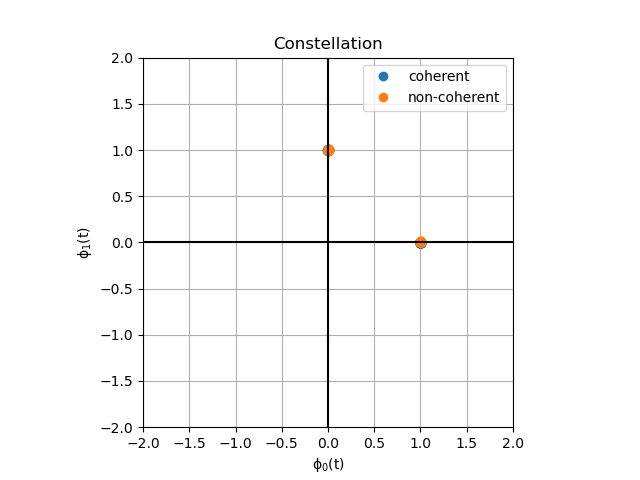
\includegraphics[width=1.2\textwidth]{phase_offset0.png} % Include the figure
	\caption{Phase Offset, Theta = [0,0]}
	\label{fig:block}
\end{figure}

\begin{lstlisting}
	Theta: [0, 0]
	Symbol error rate (coherent demod) (%):  0.0
	Symbol error rate (non-coherent demod) (%):  0.0
\end{lstlisting}

\begin{figure}[H] % [H] forces the figure to be placed exactly where it appears in the text
	\centering % Horizontally center the figure
	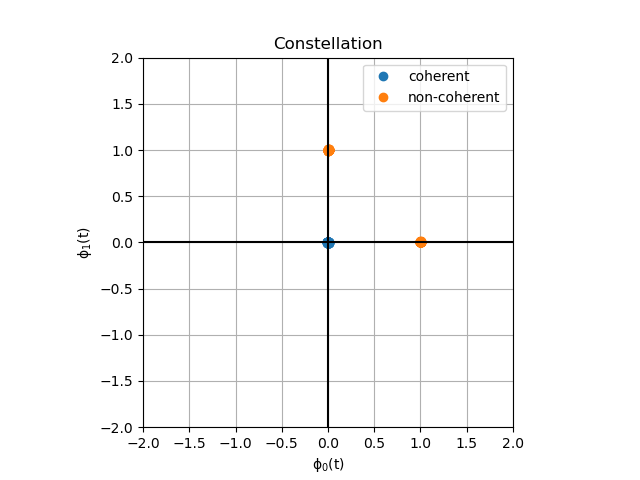
\includegraphics[width=1.2\textwidth]{phase_offset1.png} % Include the figure
	\caption{Phase Offset, Theta: [1.5707963267948966, 1.5707963267948966]}
	\label{fig:block}
\end{figure}

\begin{lstlisting}
	Theta: [1.5707963267948966, 1.5707963267948966]
	Symbol error rate (coherent demod) (%):  53.125
	Symbol error rate (non-coherent demod) (%):  0.0
\end{lstlisting}

\begin{figure}[H] % [H] forces the figure to be placed exactly where it appears in the text
	\centering % Horizontally center the figure
	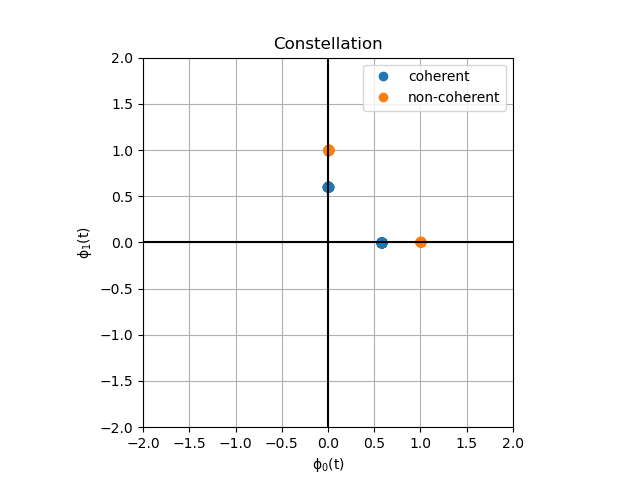
\includegraphics[width=1.2\textwidth]{phase_offset2.png} % Include the figure
	\caption{Phase Offset, Theta: [0.95227566 0.92600777]}
	\label{fig:block}
\end{figure}

\begin{lstlisting}
	Theta: [0.95227566 0.92600777]
	Symbol error rate (coherent demod) (%):  0.0
	Symbol error rate (non-coherent demod) (%):  0.0
\end{lstlisting}

\begin{figure}[H] % [H] forces the figure to be placed exactly where it appears in the text
	\centering % Horizontally center the figure
	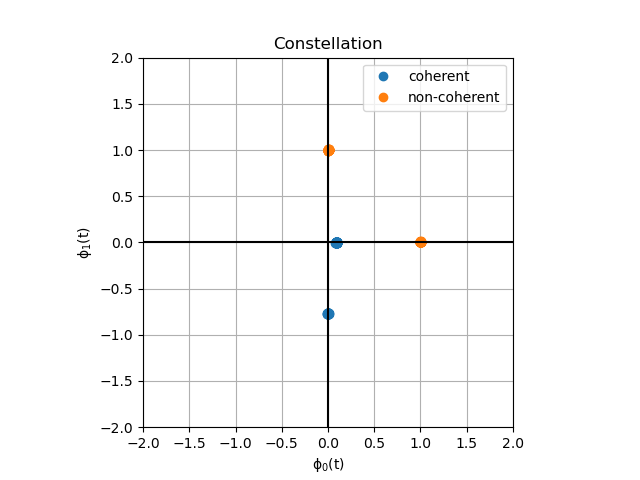
\includegraphics[width=1.2\textwidth]{phase_offset3.png} % Include the figure
	\caption{Phase Offset, Theta: [ 1.47897589 -2.44786116]}
	\label{fig:block}
\end{figure}

\begin{lstlisting}
	Theta: [ 1.47897589 -2.44786116]
	Symbol error rate (coherent demod) (%):  52.34375
	Symbol error rate (non-coherent demod) (%):  0.0
\end{lstlisting}

\begin{figure}[H] % [H] forces the figure to be placed exactly where it appears in the text
	\centering % Horizontally center the figure
	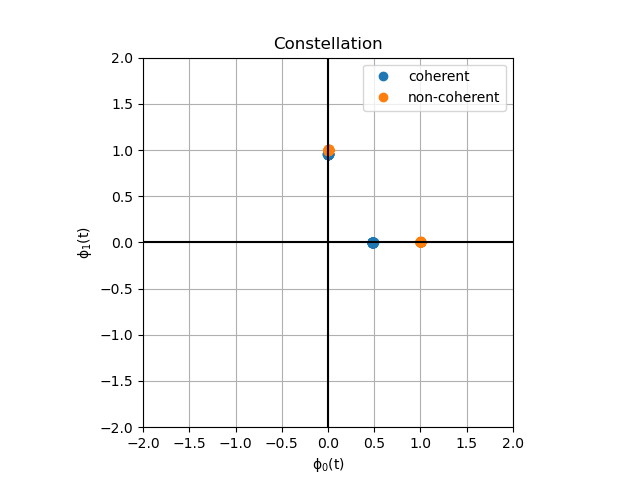
\includegraphics[width=1.2\textwidth]{phase_offset4.png} % Include the figure
	\caption{Phase Offset, Theta: [-1.06542833 -0.29993159]}
	\label{fig:block}
\end{figure}

\begin{lstlisting}
	Theta: [-1.06542833 -0.29993159]
	Symbol error rate (coherent demod) (%):  0.0
	Symbol error rate (non-coherent demod) (%):  0.0
\end{lstlisting}

Frequency Spacing Impact:

\begin{figure}[H] % [H] forces the figure to be placed exactly where it appears in the text
	\centering % Horizontally center the figure
	\includegraphics[width=1.2\textwidth]{freq\_separation0.png} % Include the figure
	\caption{Frequency Spacing, delta f = 1 / Tb}
	\label{fig:block}
\end{figure}

\begin{figure}[H] % [H] forces the figure to be placed exactly where it appears in the text
	\centering % Horizontally center the figure
s	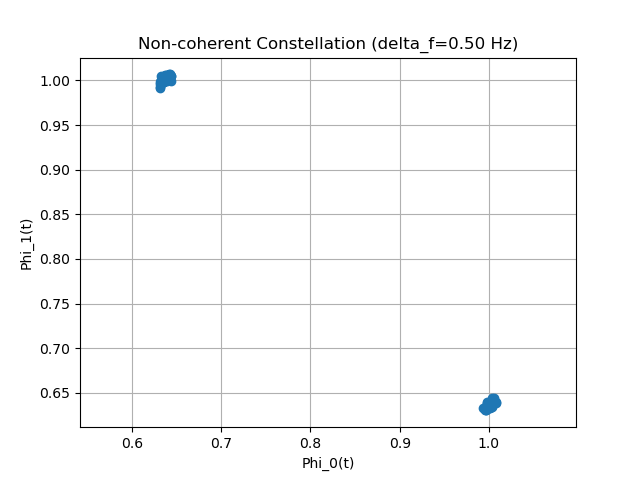
\includegraphics[width=1.2\textwidth]{freq_separation1.png} % Include the figure
	\caption{Frequency Spacing, delta f = 1 / 2*Tb}
	\label{fig:block}
\end{figure}

\begin{figure}[H] % [H] forces the figure to be placed exactly where it appears in the text
	\centering % Horizontally center the figure
	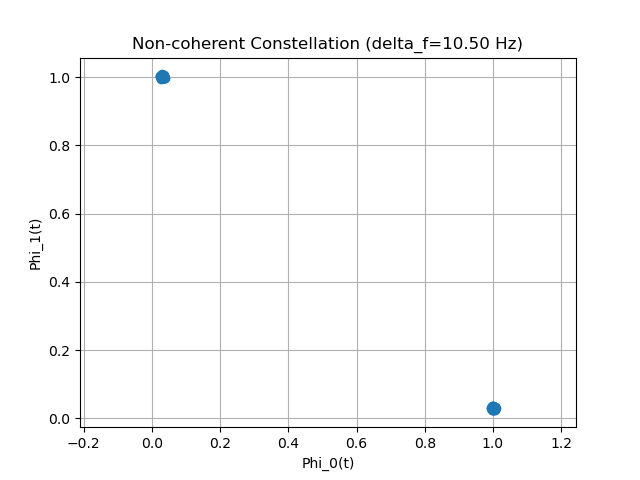
\includegraphics[width=1.2\textwidth]{freq_separation2.png} % Include the figure
	\caption{Frequency Spacing, delta f = 10.5 / Tb}
	\label{fig:block}
\end{figure}

Smaller frequency spacing like 1/(2*Tb) possibly leads to overlapping symbols and higher SER. \newline
Higher frequency spacing like 10.5/Tb consumes too much bandwidth with little to no SER improvement as compared to normal frequency spacing like 1/Tb.

\end{document}